\chapter{Introduction}
Implantable medical devices such as cardiac pacemakers and defibrillators are designed to improve physiological conditions with very little human intervention. 
Their ability to autonomously affect the physiological state of the patient makes the medical devices safety-critical, and sufficient evidence for their safety and efficacy should be provided before the devices can be implanted in the patients. Medical devices increasingly rely on software, and device function and their clinical performance can be affected by seemingly minor changes to software.

  Over the course of the past four decades, cardiac rhythm management devices such as pacemakers and implantable cardioverter defibrillators (ICD) have grown in complexity and now have more than 80,000 to 100,000 lines of code (\cite{pauljones}). According to the US Food and Drug Administration, in 1996, 10\% of all medical device recalls were caused by software-related issues. This rose to 21\% of recalls by 2006 and then to 24\% in 2011 (\cite{medstats}). Most of these recalls are categorized as \emph{Class I}, meaning there is a ``reasonable probability that use of these products will cause serious adverse health consequences or death.'' (\cite{medstats2,pacemakerrecalls,killedbycode}). While guidances and best practices exist, there is currently no standard for testing, validating and verifying the software for implantable medical devices. Given the alarming rate at which medical device software has become a safety concern, there is an urgent need for new systematic approaches and tools to evaluate the safety of software in such devices. 

Software embedded in a medical device, unlike electrical and mechanical components, does not fail due to corrosion, fatigue or have statistical failures of subcomponents. Software failures are uniquely sourced in the design and development of the system. Unlike other industries such as consumer electronics where product life cycles are measured in months, software engineering for medical devices often spans a decade and must prioritize safety and efficacy over time to market. The medical device industry is a regulated industry. The regulatory oversight reaches much further than a review of test results in a manufacturer's premarket submission and into every stage of the development process. Regulatory oversight also governs \emph{how} the device was developed, not just \emph{what} it turned out to be. The belief is that a well-planned, systematic engineering process produces more reliable devices, especially if software is a component of the device (\cite{med-book}).

In safety-critical industries such as automotive electronics, avionics and nuclear systems, standards are enforced for safe software development, evaluation, manufacturing and post-market changes (\cite{autosar,avsi}). This awareness is only beginning to enter the medical device industry (\cite{formal_fda}). However, the medical domain presents its own unique set of challenges:\\
\textbf{1. Closed-loop context:} Current evaluation of devices is open-loop and is unable to ensure the device never drives the patient into an unsafe state. Medical device testing and validation must thus be within the closed-loop context of the patient physiology. The context of the patient is a function of both the environment and the input from the device controller and must be captured by the device evaluation process.\\ 
\textbf{2. Patient models:} There is a scarcity of patient models and clinically-relevant simulators for device design (\cite{pat-model}). High-fidelity models of interaction between the patient and device are needed to evaluate the safety and efficacy of device operation. Furthermore, these models must integrate the functional and formal aspects so that testing and verification are evaluated for the same patient states.\\
\textbf{3. Adaptive patient-specific algorithms:} The therapy offered by the device must adapt to the environment and specific patient's condition. There is a need for validation algorithms to ensure that device control and optimization can cover large classes of patient conditions. 

\section{The FDA and Medical Device Software}
Before we delve into the current state of medical device software, it is useful to understand the evolution of the regulatory environment. The United States Food and Drug Administration (FDA) is the primary regulatory authority responsible for assuring the safety, efficacy and security of patients using medical devices. The history of the FDA is a reactionary one, where each stage of evolution was in response to a major healthcare tragedy. 

Through the course of the 1980s, software began to play an increasing role in medical devices. Software, as it turns out, is one of those technologies not anticipated by prior regulation, and was waiting for its disaster to prompt regulatory action. It wasn't until the 1980s when a number of cancer patients received massive X-ray overdoses during radiation therapy with the Therac-25 linear accelerator. This lead to a number of investigations, perhaps the most thorough of which was that of \cite{therac}, which was rich with identified ways software could go wrong. Inadequate testing, dangerous code reuse, configuration management issues, inadequate manufacturer response, and failure to get to the root cause of the problem were among the leaders of the problems identified. The Therac-25 was an eye-opener for the FDA and legislators, and resulted in the Safe Medical Device Act of 1990. This finally required closer medical device tracking, post-market surveillance and recommendations on development, testing and validation of medical device software. 

The FDA currently does not request or review the medical device software during pre-market submission. While no specific requirements or software verification standards are issued, a set of general guidelines for software evaluation are recommended (\cite{fda1, fda2, fda3}). The responsibility to test, validate and verify the device software to demonstrate its safety and efficacy is solely on the manufacturer. This is currently satisfied by the documentation of code inspections, static analysis, module-level testing and integration testing and their purpose is to establish ``reasonable assurance of safety and effectiveness''. These tests however fail to check for the correctness of the software and are largely open-loop tests that do not consider the context of the patient. Software is reviewed by the FDA only in the incident of a device recall. Software-related recalls are often issued in the form of \emph{Safety Alerts} by the %%%%%Food and Drug Administration (FDA) 
FDA such as ``Safety alert - Pacemaker may revert to VVI mode at 70 beats/min if programmed to one of several specific ventricular pulse widths" (\cite{medstats}).

According to their potential risks the devices are categorized into 3 classes, Class I, Class II and Class III, corresponding to low-risk, medium-risk and high-risk devices \cite{class}. Life-sustaining devices like implantable pacemakers are classified as Class III and in general are subject to the most strict regulations.

There are two processes through which a medical device can enter the market in U.S.: the Premarket Notification, also known as 510(k) \cite{510k}, and the Pre-Market Approval (PMA) \cite{PMA}. In a 510(k) submission the device manufacturers are only required to provide evidence that the device is \emph{substantial equivalent} to a \emph{predicate device}, which has been approved for the market. Therefore, the 510(k) submission does not directly require clinical evidence for the safety and effectiveness of the device, thus is suitable for mostly low-risk devices like Class I and Class II devices.  The Pre-Market Approval (PMA) submission is a more stringent regulatory process in which direct clinical evidence is required to prove the safety and effectiveness of the device. However, not all Class III devices are subject to PMA submission. If a Class III device clears the 510(k) process and FDA has not requested PMA for that device, the device is still cleared for market release. A study shows that for Class III devices which PMA has been requested, the levels of evidence varies. Only 40\% of the PMA submissions are supported by controlled clinical trials, which provide the most rigorous clinical evidence \cite{cert_prob}. The lack of quality evidence is usually due to the high cost of the controlled clinical trials.
\begin{figure}[b]
		\centering
		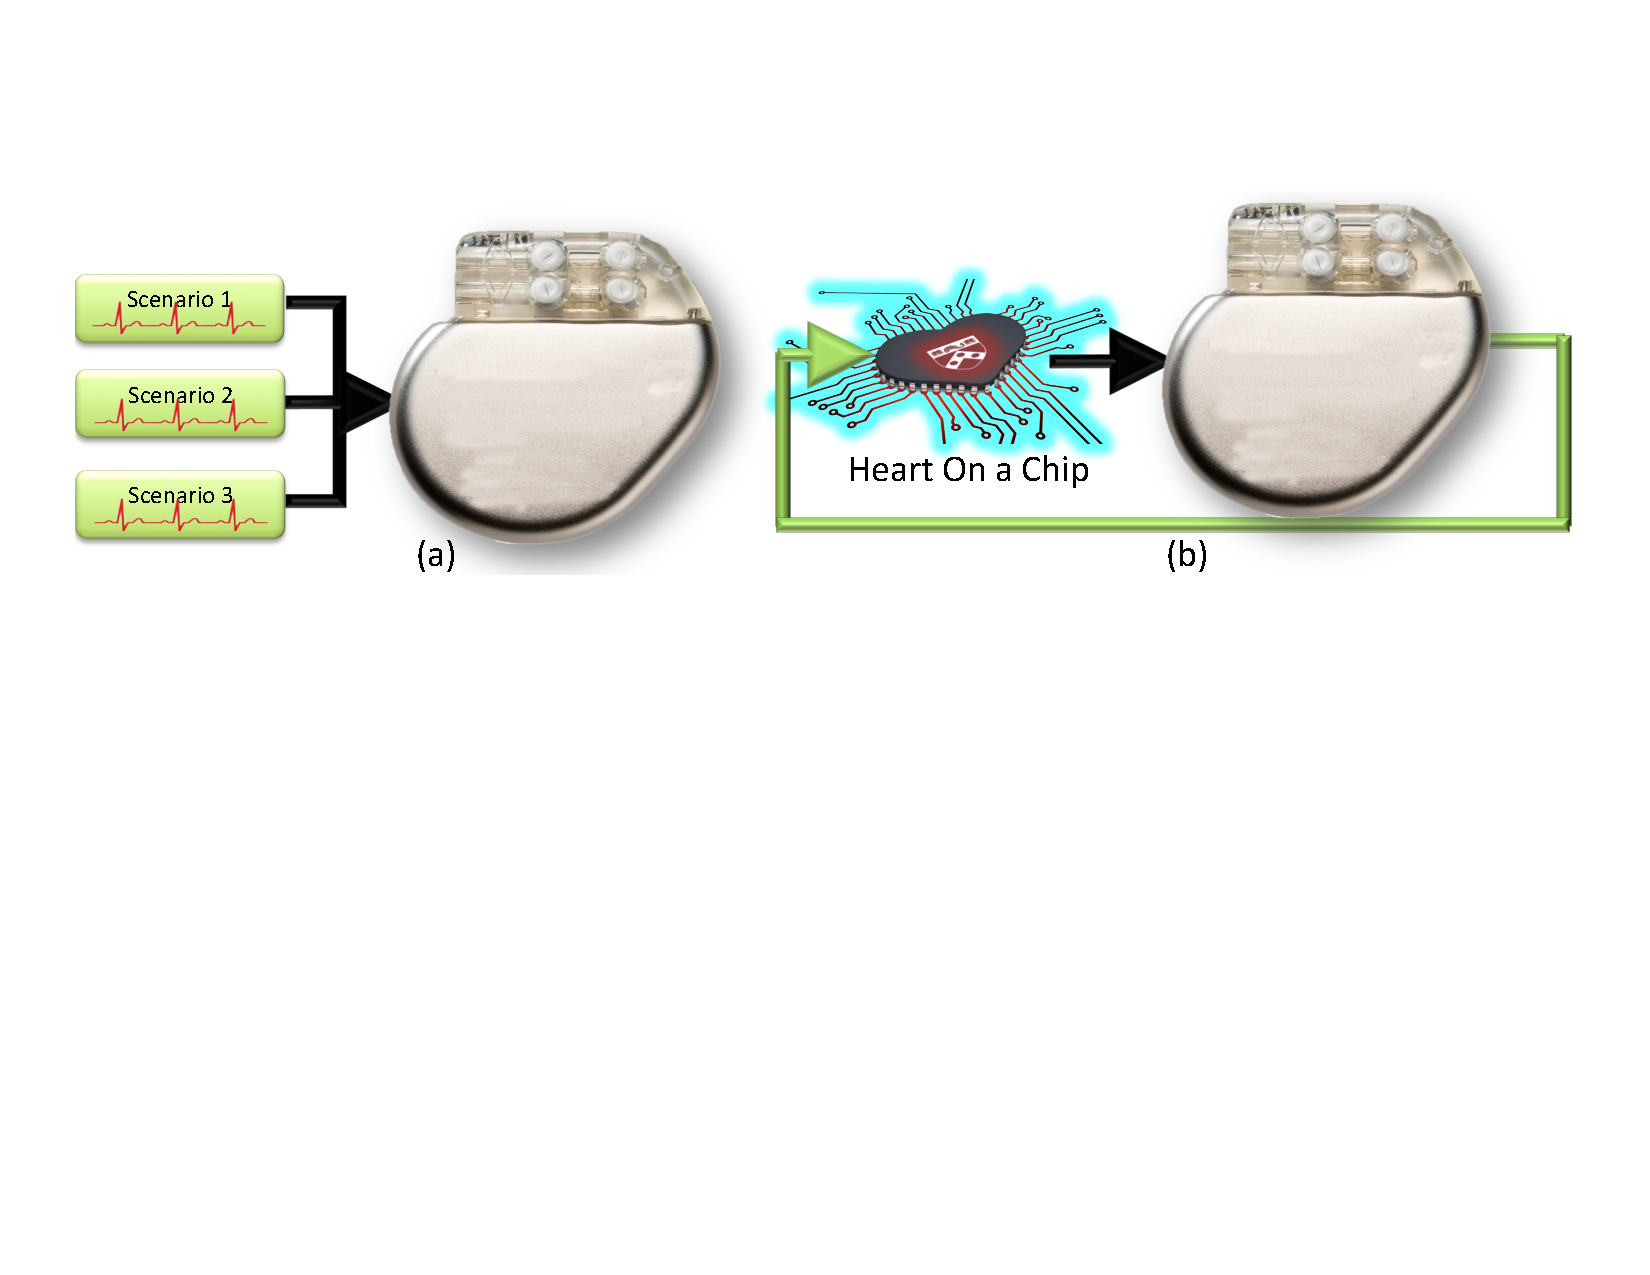
\includegraphics[width=0.9\textwidth]{figs/closedloop.pdf}
		\caption{\small (a) The current practice of open loop testing of the pacemaker. (b) The desired closed-loop verification of a model of the pacemaker and model of the heart and testing of the real pacemaker with a heart-on-a-chip platform}
		\label{fig:closedloop}
\end{figure}
\section{Current Testing, Validation and Verification Approaches}
In order to facilitate the early detection and correction of any software defects, the FDA has focused on infusion pumps due to the large number of recalls. In April 2010, the FDA began the ``Infusion Pump Improvement Initiative" which offers manufacturers ``the option of submitting the software code used in their infusion pumps for analysis by agency experts prior to premarket review of new or modified devices." 	

An effective software verification methodology is therefore needed for the risk analysis and certification of medical device software during the pre-market submission phase. While formal methods of verification are used for medical device software (\cite{challenge, challenge2, challenge3}), testing continues to be required because it can expose different kinds of problems (e.g. compiler bugs), can examine the program in its system context, and increases the diversity of evidence available. Testing for medical device software currently is ad hoc, error prone, and very expensive. Traditional methods of testing do not suffice as the test generation cannot be done independently of the current state of the patient and organ. The primary approach for system-level testing of medical devices is unit testing using a playback of pre-recorded electrogram and electrocardiogram signals (\cite{testing_imd, Vip}). This tests if the input signal triggers a particular response by the pacemaker but has no means to evaluate if the response was appropriate for the patient condition. Furthermore, this approach of ``tape testing'' is unable to check for safety violations due to inappropriate stimulus by the pacemaker. Pacemaker Mediated Tachycardia (PMT), a condition that is described later in this paper, is a strong example of why we need a model of the heart such as the one presented in this paper, which can be used for closed-loop system analysis. 
PMT is a condition where the pacemaker inappropriately drives the heart-rate toward the upper rate limit. With a tape test, PMT would not occur and the response of the pacemaker could be classified as appropriate therapy.
\begin{figure}[t]
		\centering
		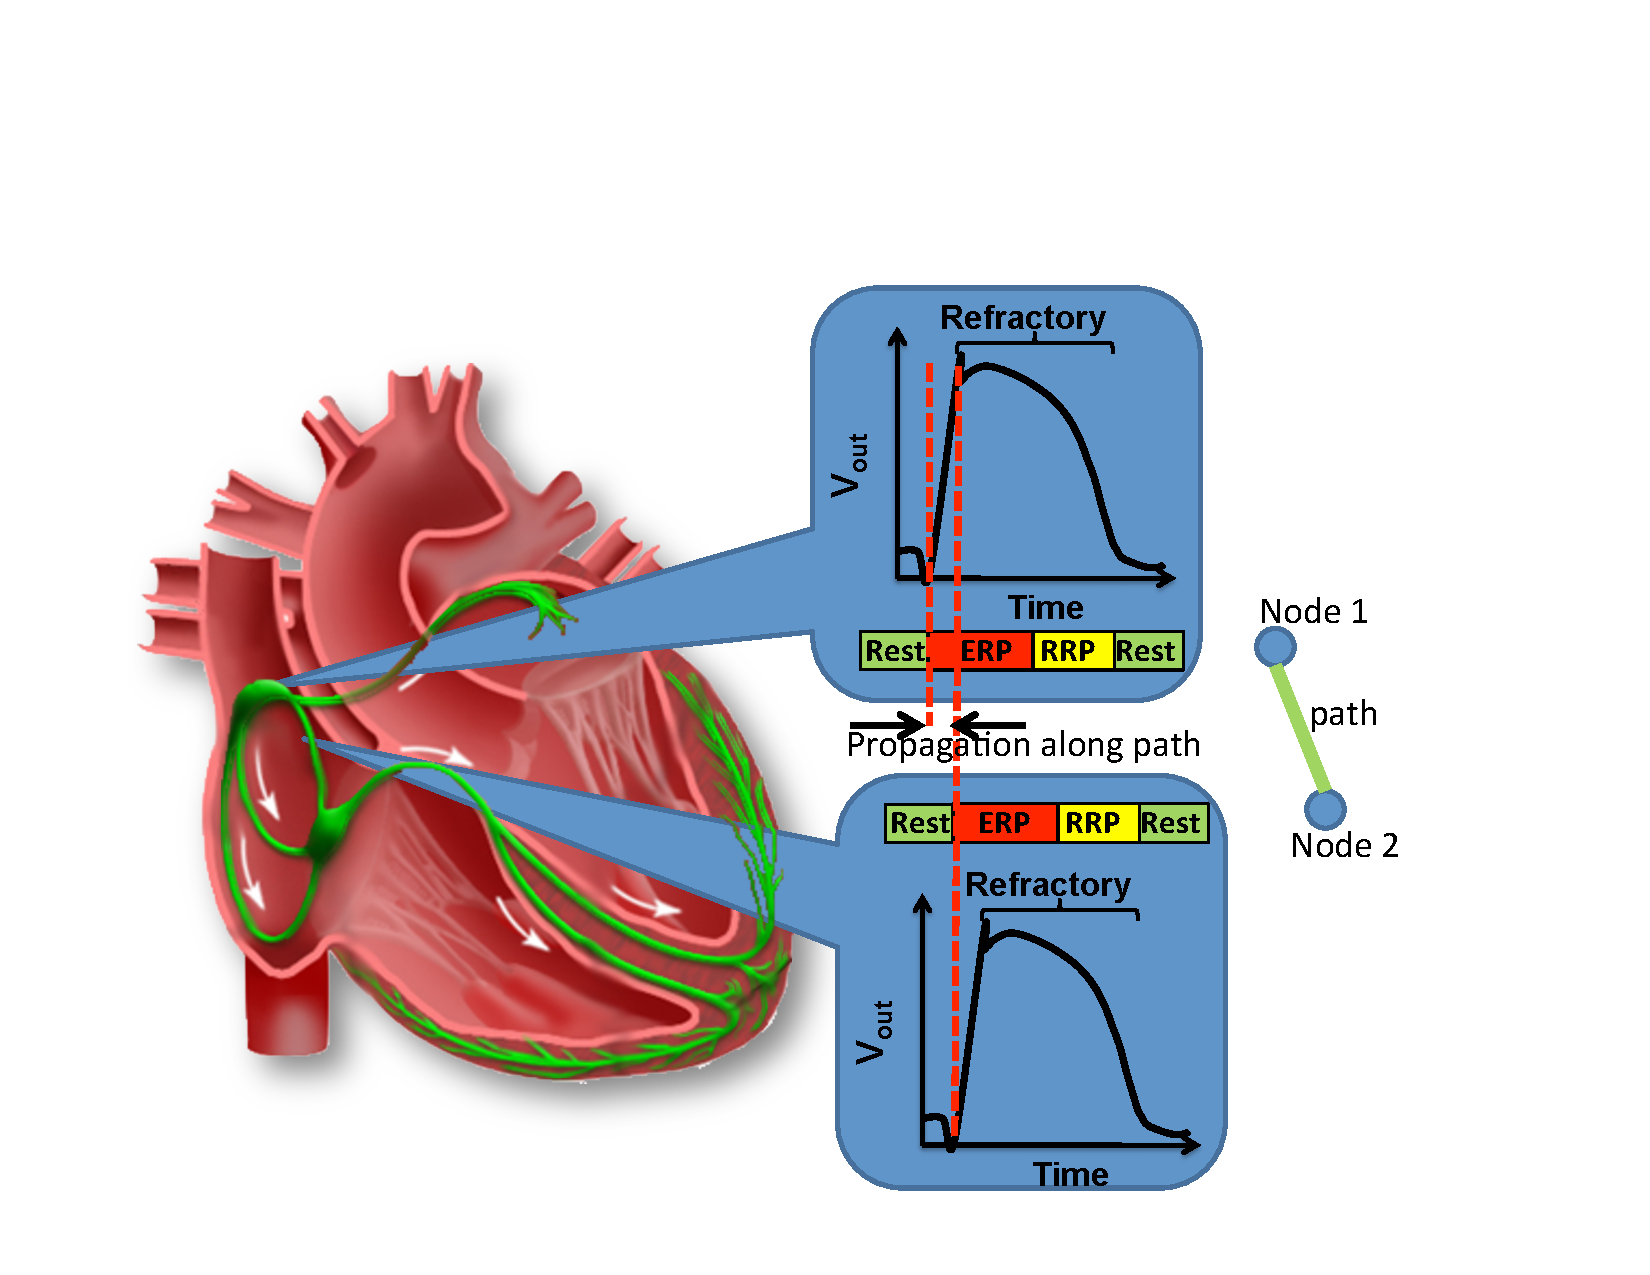
\includegraphics[width=0.8\textwidth]{figs/heartmodel.pdf}
		%\vspace{-5pt}
		\caption{\small By extracting timing and electric conduction information we model the signal activation, refractoriness and propagation across the heart tissue as a set of node and path automata.}
		  %\vspace{-15pt}
		\label{fig:heartmodel}
\end{figure}
As the testing environment (i.e., patient condition) is not entirely under the control of the tester, the problem changes significantly as a degree of nondeterminism is introduced in the process. Implantable medical devices are a primary example of Medical Cyber-Physical Systems where the safety and efficacy of the device and device software must be evaluated within a closed-loop context of the patient. The key challenge is in the generation of physiologically relevant tests such that the device does not provide inappropriate therapy and does not adversely affect the safety of the patient. In addition, test generation must be interactive and adaptive such that the previous test stimulus affects the current state of the patient. The test generator must consider the current state when generating the next input in a way that advances the purpose of the test. The problem becomes one of the controller synthesis problems and cannot be addressed by an off-the-shelf model checker~\cite{rushby}.  
   
Formal methods have traditionally been used for verification of time-critical and safety-critical embedded systems \cite{form-meth}. Until recently, these methods have not been used for medical device certification. \cite{med-form3} presented the use of Extended Finite State Machines for model checking of a resuscitation device. Formal techniques have also been applied to improve medical device protocols (\cite{med-form2}) and safety (\cite{med-form1}), but the authors either used a simplified patient model or did not model the patient at all. 

\section{Methodology for Closed-loop Medical Device Safety}
The focus of this effort is three-fold: (a) We developed an integrated functional (i.e., clinically-relevant) and formal (i.e., timed automata based) Virtual Heart Model  (VHM) (see \figref{heartmodel}) and a pacemaker device model for interactive and clinically relevant test generation.  (b) We provide a set of general and patient condition-specific pacemaker software requirements to ensure the safety of the patient is met under all cases, and (c) We provide a means to test and verify the closed-loop system over a variety of basic operation tests where the heart rate must be maintained, the atrial-ventricle synchrony must be enforced and complex closed-loop tests, where the pacemaker must not initiate tachycardia or perform improperly during lead displacement. With this approach of model-based testing, an executable functional model of the pacemaker is created at an early stage in the development process. This model-based methodology is an early step in addressing the urgent need for pre-market evaluation of medical device design and certification.

Our proposed model-driven design (MDD) for Medical CPS begins with developing integrated functional and formal heart models that interact with real and modeled pacemakers for closed-loop verification and testing (\cite{VHM_proc}). As shown from the top of \figref{modeling_overview}, the heart-pacemaker closed-loop systems is first modeled abstractly to facilitate verification of the basic pacemaker design with maximum coverage (\cite{STTT13}). In our case, we use timed automata and the UPPAAL model checker at this design stage. Next, the models are translated to more detailed models that take into account the complex dynamics of the heart and interaction with more detailed pacemaker model (\cite{vhm_ecrts10, vhm_embc11,vhm_iccps11}). We use Stateflow and Simulink at this design stage. These models are validated by physicians for their clinical relevance. The automatic model translation procedure, from UPPAAL to Stateflow, ensures that abstract models used for verification over-approximate the more detailed models used downstream (\cite{RTAS12}). Once the detailed models pass simulation-based testing with closed-loop dynamics, they are automatically generated into code and are subject to platform-level integration testing (\cite{vhm_website}). This MDD approach ensures the closed-loop safety properties are retained through the design toolchain and facilitates the development of verified software from verified models.
\begin{figure}[t]
		\centering
		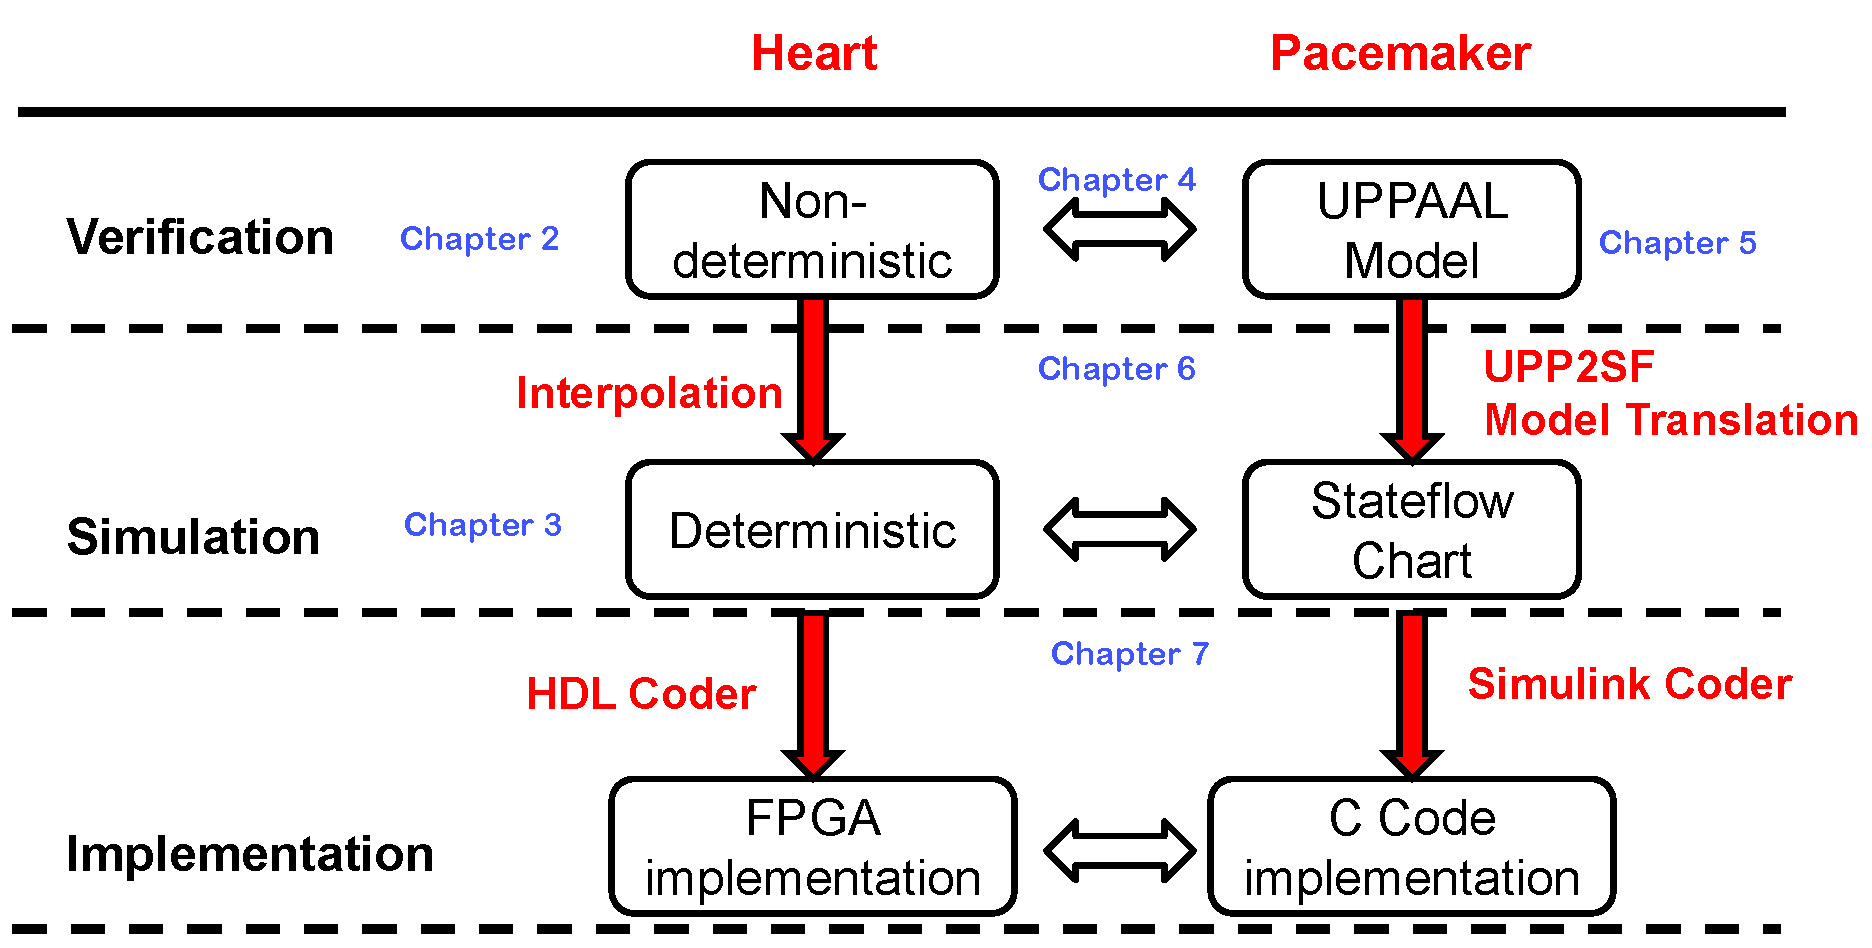
\includegraphics[width=0.8\textwidth]{figs/modeling_overview.jpg}
		%\vspace{-5pt}
		\caption{\small Model-driven design for verified models to verified code for the closed-loop heart and pacemaker system}
		  %\vspace{-15pt}
		\label{fig:modeling_overview}
\end{figure}
%%Through each of the chapters to follow, we cover different aspects of modeling the physiological system and the device, validating the models, running model checking on the closed-loop system and testing the deterministic systems derived from the abstract models. With the goal of 
